\documentclass{examen}

\begin{document}
\modulo{Lenguajes de marcas -- PARTE ORDENADOR (PARTES 1 y 2)}


\pregunta{Crea un formulario como el mostrado en la figura}{2}
\begin{figure}[h]
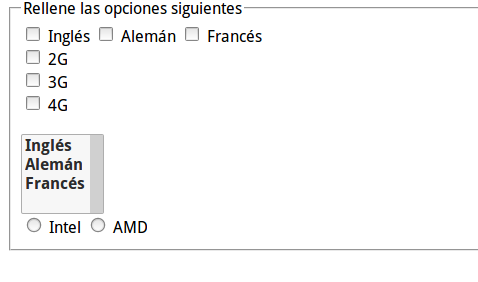
\includegraphics[scale=0.7]{examen-img/pagina.png}
\end{figure}
\break

\pregunta{Crear un esquema XML que permita validar un fichero como el que se muestra a continuaci�n. Se muestran a continuaci�n los requisitos}{3}
\begin{itemize}
\item{    La ra�z se llama {\tt listado}.}
\item{    Dentro de la lista debe haber uno o m�s elementos {\tt cliente}.}
\item{    Todos los clientes tienen siempre un atributo {\tt id}. Este atributo tiene siempre la misma estructura: dos may�sculas, seguidas de un gui�n, seguido de dos cifras.}
\item{    Todos los clientes tienen siempre dos elementos {\tt nombre} y {\tt pago}.}
\item{    El {\tt nombre} siempre es una cadena de texto}
\item{    El pago tiene siempre un atributo {\tt moneda}. Este atributo siempre vale uno de estos dos valores: ``euros'' o ``dolares''}
\item{    Dentro del elemento {\tt pago} siempre hay un elemento {\tt cantidad}, que es siempre un numero entero positivo. Despues de la cantidad puede haber o no un elemento {\tt banco} que es siempre una cadena de texto}

\end{itemize}

\begin{verbatim}
<!--Ejemplo de fichero-->
<listado>
    <cliente id="AZ-89">
        <nombre>Juan Sanchez</nombre>
        <pago moneda="euros">
            <cantidad>210</cantidad>
            <banco>Caja de ahorros</banco>
        </pago>
    </cliente>
    <cliente id="AZ-89">
        <nombre>Tomas Ruiz</nombre>
        <pago moneda="dolares">
            <cantidad>460</cantidad>
        </pago>
    </cliente>
</listado>
\end{verbatim}
\end{document}
